L'astronomia nasce dall'osservazione del moto degli oggetti in cielo. Questo ha portato alla definizione di \textbf{tempo} e alla nascita degli attuali sistemi di riferimento. Il tempo è stato definito tramite il sorgere e il tramontare del sole per scandire le giornate. Questo ha portato alla nascita delle meridiane, uno dei primi strumenti per misurare oggettivamente il tempo.

La durata del \textbf{giorno solare} è stata definita come il tempo che il Sole impiega a rioccupare la stessa posizione relativamente alla Terra, ed è stato poi suddiviso in 24 ore.

Ciò vale per il Sole, ma non per le altre stelle: se osservassimo il moto di una stella attorno alla polare (l'asse passante per il polo), ci accorgeremmo che non impiega 24 ore, bensì 23 ore 56 minuti e 4.1 secondi; questa è la durata del \textbf{giorno siderale}.

\begin{figure}[h!]
   \centering
   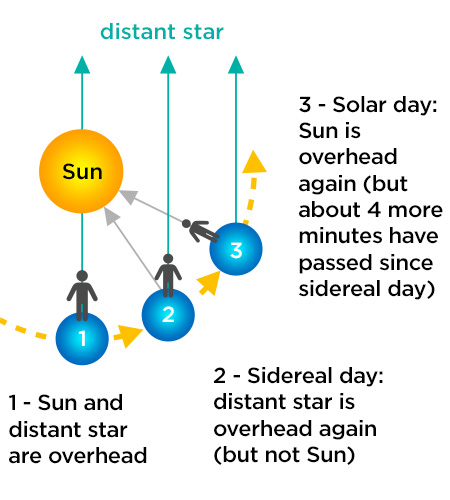
\includegraphics[width=8 cm]{immagini/giorno_solare_e_siderale.png}
\end{figure}

Questo ha portato alla comprensione che era la Terra a girare intorno al Sole, e che la differenza fra giorno solare e siderale è dovuta all'orbita della Terra.

Analogamente è stato definito l'\textbf{anno sidereo} come il tempo che deve trascorrere affinché il sole rioccupi la stessa posizione rispetto alle stelle. Il Sole nel suo moto apparente passa attraverso alcune costellazioni chiamate costellazioni zodiacali. L'anno sidereo dura 365 giorni 6 ore 9 minuti e 9.54 secondi; per comodità si usa solo la parte intera e ogni quattro anni si aggiunge un giorno (anno bisestile).

Gli astronomi preferiscono utilizzare le frazioni del giorno, cioè l'unità è rappresentata dal giorno, e come zero dell'asse dei tempi si è scelta la \textbf{data giuliana}, la quale è il numero di giorni trascorsi a partire dalle ore 12:00 nel meridiano di Greenwich dell'1 gennaio del 4713 a.C.\,. La data giuliana cambia a mezzogiorno, in modo tale che così non cambia la data durante la stessa notte di osservazione.
%Questo metodo da una continuità al tempo. È stato proposto il 4713 il Sole, a causa della precessione, si trovava nell'esatto punto quando lui aveva fatto la proposta; in realtà venne accolta perché non c'è nessuna traccia astronomica prima di tale data.

Osservando il cielo dell'emisfero boreale ci si è resi conto che l'altezza del Sole in estate è molto più alta che in inverno. Da ciò si è dedotto che l'asse di rotazione della Terra è inclinato rispetto all'orbita terrestre, e in conseguenza a ciò con il variare dell'altezza del Sole cambiano le stagioni. In particolare l'inclinazione dell'asse terrestre è di $23.45^\circ$.